\chapter{Описание принципа работы подсистемы измерения энергопотребления}
\section{Обоснование выбора компонентов измерительной части}
\subsection{Операционный усилитель}
\hspace{1cm} 

В измерительной схеме будем использовать дифференциальный усилитель, который позволит нам реализовать
двунаправленный измеритель тока, например как в схеме, изображенной на рисунке 
\ref{ris:Bidirectional cur sense} \cite{Bidirectional cur sense}. 

\begin{figure}[H]
\centering
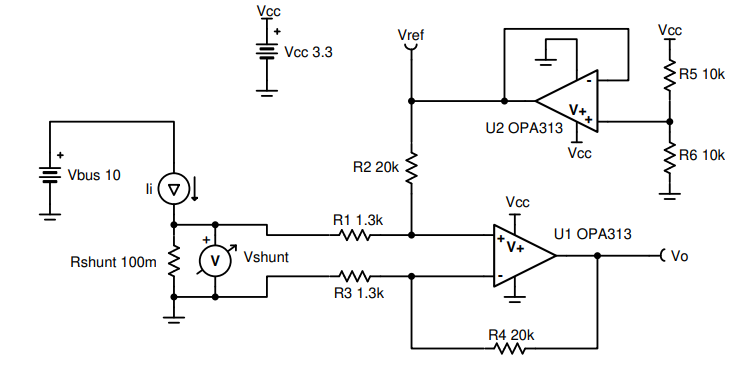
\includegraphics[scale = 0.8]{Bidirectional cur sense.png}
\caption{Двунаправленный измеритель тока}
\label{ris:Bidirectional cur sense}
\end{figure}

Не будем подробно рассматривать эту схему, так как подобная ей будет использоваться в нашем устройстве,
описание работы которой будет приведено ниже.

Вопрос какой операционный усилитель (далее ОУ) использовать в качестве дифференциального усилителя -- самый 
критичный для подсистемы измерения энергопотребления. Прежде всего стоит определиться с требованиями к 
самым важным параметрам ОУ. 
Одной из важных характеристик операционного усилителя (ОУ) является напряжение смещения $V_{os}$ — или, 
говоря проще, напряжение ошибки на его входах. Любой неидеальный ОУ при отсутствии входного сигнала выдаёт 
выходной так, как будто бы на самом деле входной сигнал равен Vos.

Напряжение смещения обычно составляет от единиц микровольт до единиц милливольт — и, соответственно, 
доставляет серьёзные неудобства при работе с низковольтными источниками: термопарами, шунтами и так далее.
Особенно — если оно отрицательное, а схема однополярная: тогда на выходе ОУ будет просто 0, пока 
напряжение входного сигнала не превысит Vos, и никакой калибровкой это устранить невозможно \cite{Chopper:OU} 
\cite{MT-037:Tutorial}. 

При измерении микро- и миллиамперных диапазонов высокое напряжение смещения может стать проблемой.
Для этого следует изучить реальную зависимость напряжения смещения от Vcm, -- синфазного
напряжения на входах ОУ, и сравнить ее с той, 
которую приводят в datasheet, как, например, на рисунке \ref{ris:411} \cite{OPAx376:datasheet}.
\begin{figure}[H]
\centering
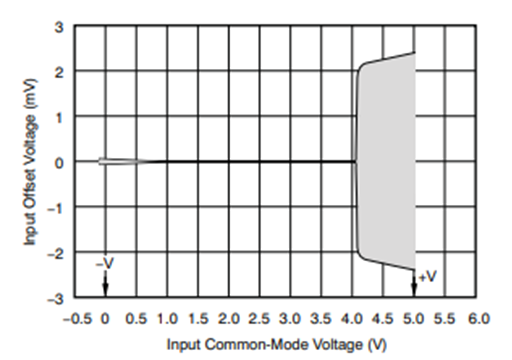
\includegraphics[scale = 0.8]{ris411.png}
\caption{Зависимость напряжения смещения от $V_{cm}$}
\label{ris:411}
\end{figure}

Так же стоит посмотреть на напряжение смещения в зависимости от ОУ в партии, 
на рисунке \ref{ris:412} представлен график для OPA2376 \cite{OPAx376:datasheet}

\begin{figure}[H]
\centering
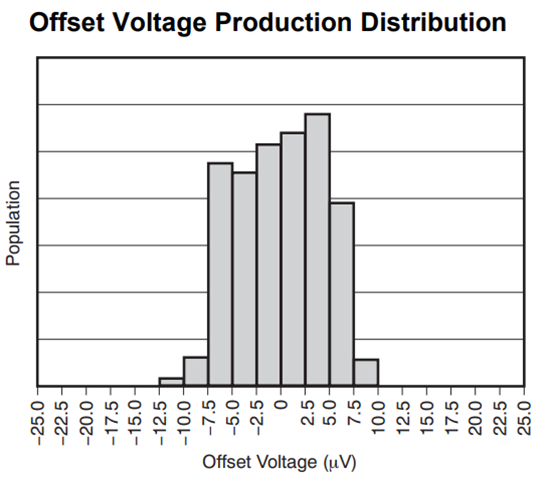
\includegraphics[scale = 0.8]{ris412.png}
\caption{Показатель напряжения смещения в рамках одной партии}
\label{ris:412}
\end{figure}

Для получения наименьшего $V_{os}$ очень хорошо подходят чоппер-стабилизированные ОУ. Они имеют напряжение 
смещения менее 5 мкВ при практически полном отсутствии измеряемого дрейфа. 

Принцип работы чоппер-стабилизированных ОУ показан на рисунке \ref{ris:ChopperOP} \cite{MT-055:Tutorial}.

\begin{figure}[H]
\centering
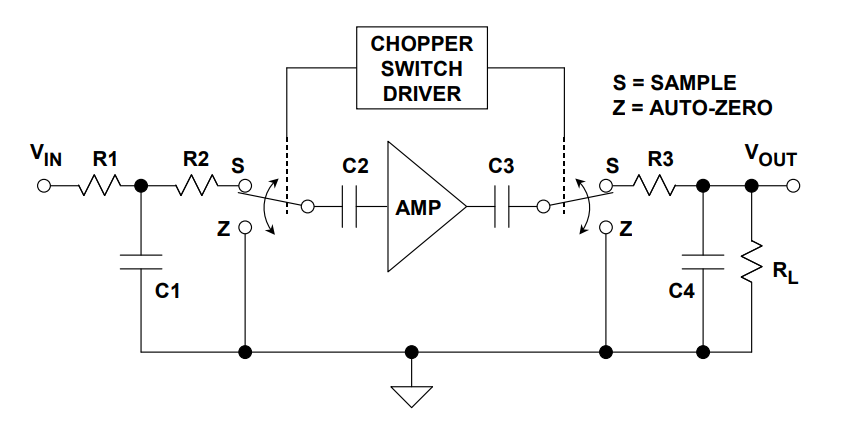
\includegraphics[scale = 0.8]{ChopperOP.png}
\caption{Типичная схема чопперного ОУ}
\label{ris:ChopperOP}
\end{figure}


Когда переключатели находятся в положении <<Z>>, конденсаторы C2 и C3 заряжены до входного и выходного
напряжения смещения усилителя, соответственно. Когда переключатели находятся в положении <<S>>, 
VIN соединяется с $V_{out}$ через канал, состоящий из R1, R2, C2, усилителя, C3 и R3. Комбинация R1-C1 служит в 
качестве фильтра сглаживания. Также предполагается, что после достижения устойчивого состояния во время 
циклов переключения передается лишь минимальное количество заряда. Выходной конденсатор C4 и нагрузка $R_{L}$ 
должны быть подобраны таким образом, чтобы во время цикла автообнуления наблюдался минимальный спад $V_{out}$ 
\cite{MT-055:Tutorial}.

Также стоит упомянуть про то, что при использовании автоматического переключения шунтов 
чоппер-стабилизированные ОУ могут быть малопригодны из-за долгого времени восстановления, 
так как из-за частоты работы
АЦП порядка сотен кГц, время переключения свыше 1 мкс нам не подходит \cite{Chopper:OU}.

Другой технологией операционных усилителей с малым напряжением смещения является DigiTrim (в терминологии Analog 
Devices) или E-Trim (в терминологии Texas Instruments).

Базовая схема таких ОУ изображена на рисунке \ref{ris:DigiTrim} \cite{MT-037:Tutorial}.

\begin{figure}[H]
\centering
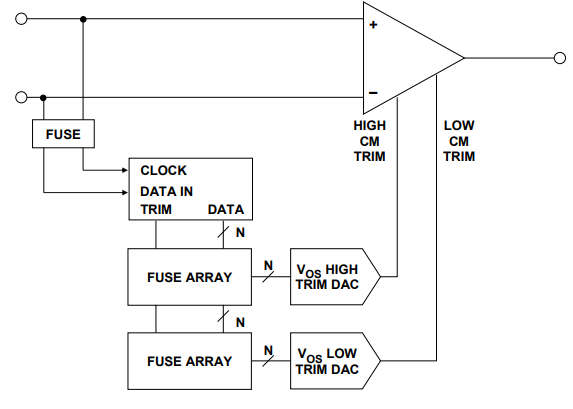
\includegraphics[scale = 0.9]{DigiTrim.png}
\caption{Типичная схема DigiTrim ОУ}
\label{ris:DigiTrim}
\end{figure}

DigiTrim регулирует напряжение смещения путем программирования источников тока с цифровым взвешиванием. 
Информация о подстройке вводится через существующие контакты с помощью специальной цифровой последовательности. 
Значения регулировки могут быть временно запрограммированы, оценены и скорректированы для достижения 
оптимальной точности перед выполнением постоянной регулировки. 
После завершения настройки схема настройки блокируется, чтобы исключить возможность случайной повторной 
настройки конечным пользователем \cite{MT-037:Tutorial}. 

Исходя из вышесказанного, можно изучить следующие ОУ:

\begin{itemize}
    \item OPA2376 от Texas Instruments -- прецизионный rail-to-rail, выполненный по технологии etrim
    \item OPA2376 от Fulihao -- в ходе дальнейших экспериментов было выяснено, что это 
    чоппер-стабилизированный ОУ
    \item AD8606 от Analog Devices -- прецизионный rail-to-rail, выполненный по технологии etrim
    \item TP2312 -- прецизионный малошумящий rail-to-rail
    \item RS8552 -- чоппер-стабилизированный
    \item RS8562 -- чоппер-стабилизированный
\end{itemize}

На выбор ОУ влияла так же возможность быстро и без проблем приобрести на территории РФ. 

На рисунке \ref{ris:413} представлена схема измерения напряжения смещения, выполненная согласно
ГОСТ 23089.3-83 \cite{Simple Op Amp Measurements} \cite{GOST 23089.3-83}.

\begin{figure}[H]
    \centering
    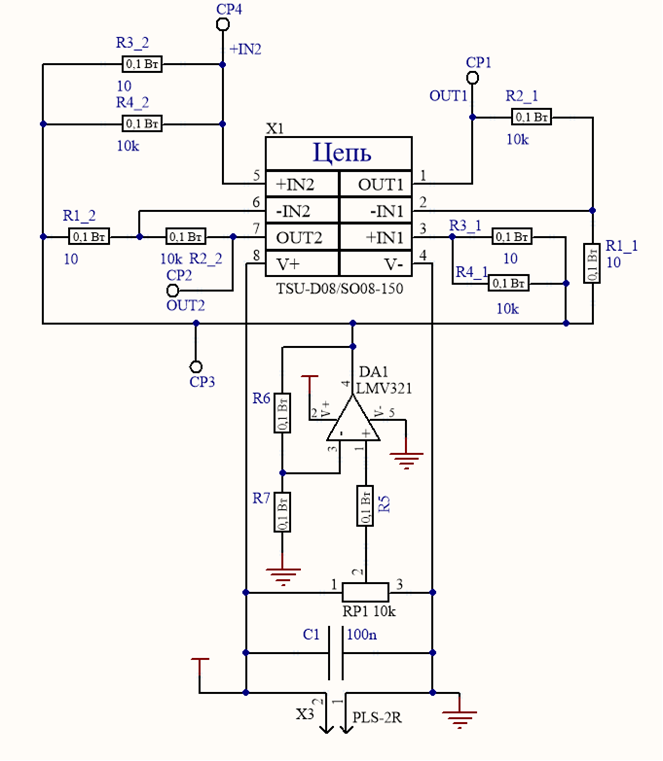
\includegraphics[scale = 0.9]{ris413.png}
    \caption{Схема измерительной установки}
    \label{ris:413}
    \end{figure}

Здесь Х1 -- контактирующее устройство, предназначенное для быстрой смены операционного усилителя в 
корпусе SOIC-8 -- самого распространённого типа корпуса для ОУ. Испытуемый ОУ включён по схеме неинвертирующего 
усилителя с коэффициентом усиления 1000, который обеспечивается резисторами R2\_1 и R1\_1 для первого ОУ и
резисторами R2\_2 и R1\_2 для второго ОУ в корпусе. DA1 с обвязкой к нему выполняет роль буферного ОУ для 
обеспечения лучшего импеданса и большей нагрузочной способности при низком токе через делитель R3 и R4.

Данная схема позволит преобразовать микровольтное напряжение смещения в милливольты, что достаточно для 
измерения обычным вольтметром. Подстроечным резистором RP1 регулируется синфазное напряжение
(input common-mode voltage), как 
на рисунке \ref{ris:411}. Напряжение питание схемы 5 В. Результаты измерений представлены в таблице
\ref{tab:Vcm1} для OPA2376 производства TI и Fulihao, AD8606 и TP2312, и в таблице \ref{tab:Vcm2} 
для RS8552 и RS8562.

% Table generated by Excel2LaTeX from sheet 'Vcm' and from my teardrops
\begin{table}[H]
    \begin{adjustwidth}{-1em}{}
    \centering
    \caption{Результаты измерений напряжения смещения у разных ОУ}
      \begin{tabular}{|c|c|c|c|c|c|c|c|c|c|c|c|}
      \hline
      \multicolumn{1}{|c|}{\multirow{3}[6]{2cm}{\textbf{Тип ОУ}}} & \multicolumn{1}{c|}{\multirow{3}[6]{1.4cm}{\textbf{Номер экземпляра}}} & \multicolumn{1}{c|}{\multirow{3}[6]{1.8cm}{\textbf{Номер ОУ в корпусе}}} & \multicolumn{9}{|c|}{\textbf{Напряжение смещения, мкВ}} \bigstrut\\
  \cline{4-12}          &       &       & \multicolumn{9}{|c|}{\textbf{При Vcm, В}} \bigstrut\\
  \cline{4-12}          &       &       & \textbf{0,5} & \textbf{1} & \textbf{1,5} & \textbf{2} & \textbf{2,5} & \textbf{3} & \textbf{3,5} & \textbf{4} & \textbf{4,5} \bigstrut\\
      \hline
      \multicolumn{1}{|c|}{\multirow{10}[20]{*}{OPA2376 }} & \multirow{2}[4]{*}{1} & 1     & 13,4  & 7,9   & 2,4   & -2,4  & -8,1  & -11,8 & -15,3 & -12,8 & 483 \bigstrut\\
  \cline{3-12}          &       & 2     & 4,2   & 6     & 4,3   & 2,3   & -1    & -3,5  & -6    & -9,7  & -1813 \bigstrut\\
  \cline{2-12}          & \multirow{2}[4]{*}{2} & 1     & 28,5  & 18,7  & 9,3   & 0,3   & -8    & -15,2 & -22,7 & -58,5 & -388 \bigstrut\\
  \cline{3-12}          &       & 2     & -5,5  & -7,5  & -8,5  & -6,8  & -6,1  & -3,9  & -1,9  & -8,9  & -680 \bigstrut\\
  \cline{2-12}          & \multirow{2}[4]{*}{3} & 1     & 26,7  & 20,3  & 14,2  & 9,1   & 3,6   & -0,2  & -4,4  & -16,6 & -2230 \bigstrut\\
  \cline{3-12}          &       & 2     & -55,7 & -33,4 & -21,7 & -12,3 & -7,3  & -1,5  & 2,9   & -10,9 & -4500 \bigstrut\\
  \cline{2-12}   TI     & \multirow{2}[4]{*}{4} & 1     & -18,2 & -10,8 & -6,3  & -2,5  & 0,1   & 2,5   & 4,6   & 14,5  & -1532 \bigstrut\\
  \cline{3-12}          &       & 2     & 7,2   & 5,5   & -0,1  & -4,8  & -9,2  & -13,4 & -17,2 & -23,3 & -1517 \bigstrut\\
  \cline{2-12}          & \multirow{2}[4]{*}{5} & 1     & -18,8 & -10,4 & -4,5  & 0,2   & 3,2   & 6,3   & 8,6   & 22    & 395 \bigstrut\\
  \cline{3-12}          &       & 2     & -70,4 & -43,6 & -24,7 & -11,2 & -1,6  & 7,5   & 14,4  & 30    & 624 \bigstrut\\
      \hline
      \multicolumn{1}{|c|}{\multirow{6}[12]{*}{OPA2376}} & \multirow{2}[4]{*}{1} & 1     & -6,3  & -6,5  & -8,4  & -8,2  & -7,35 & -7,9  & -10   & -5,9  & -4,6 \bigstrut\\
  \cline{3-12}          &       & 2     & -2,8  & -2,9  & -4,5  & -4,3  & -3,1  & -3,3  & -4,7  & -2,7  & -1,7 \bigstrut\\
  \cline{2-12}          & \multirow{2}[4]{*}{2} & 1     & -6,8  & -6,8  & -9    & -9    & -8,01 & -8,9  & -10,4 & -11,8 & -10,1 \bigstrut\\
  \cline{3-12}          &       & 2     & 1,3   & 1     & -0,6  & -0,5  & 0,2   & 1,2   & -0,1  & 2     & 3,4 \bigstrut\\
  \cline{2-12} Fulihao   & \multirow{2}[4]{*}{3} & 1     & -4,6  & -4,4  & -6,4  & -6,8  & -6,4  & -6,5  & -8,5  & -7,7  & -6,2 \bigstrut\\
  \cline{3-12}          &       & 2     & -1,4  & -1,2  & -2,3  & -2,1  & -0,8  & -0,6  & -2,3  & -1,5  & 0,2 \bigstrut\\
      \hline
      \multicolumn{1}{|c|}{\multirow{10}[20]{*}{AD8606}} & \multirow{2}[4]{*}{1} & 1     & 40,1  & 36,3  & 33,7  & 33,5  & 31,3  & 30,6  & 3,5   & 6,2   & 19,8 \bigstrut\\
  \cline{3-12}          &       & 2     & 11,4  & 32,8  & 49,3  & 59,67 & 72    & 80,5  & 19,2  & -10,4 & -13,6 \bigstrut\\
  \cline{2-12}          & \multirow{2}[4]{*}{2} & 1     & 21,4  & 27,2  & 31,3  & 34,5  & 36,1  & 38,3  & 87,5  & 73,8  & 93,6 \bigstrut\\
  \cline{3-12}          &       & 2     & 12,8  & 4,6   & 0,6   & -0,3  & -2,2  & -2,1  & -94,4 & -39,9 & -46,5 \bigstrut\\
  \cline{2-12}          & \multirow{2}[4]{*}{3} & 1     & 17,8  & 34,3  & 47,5  & 59,2  & 71,8  & 84,9  & 29,7  & 29,5  & 23,6 \bigstrut\\
  \cline{3-12}          &       & 2     & -16,3 & -3,3  & 6,6   & 13,9  & 1,3   & 27,9  & 48,8  & 9,3   & 15,6 \bigstrut\\
  \cline{2-12}          & \multirow{2}[4]{*}{4} & 1     & 74,7  & 63,5  & 51,1  & 40,5  & 31,9  & 24,1  & 40,9  & 61,6  & 73,7 \bigstrut\\
  \cline{3-12}          &       & 2     & 15,3  & -6,9  & -25,1 & -38,5 & -51,4 & -64,2 & -53,8 & -17,5 & -29,4 \bigstrut\\
  \cline{2-12}          & \multirow{2}[4]{*}{5} & 1     & 59,5  & 51,8  & 41,9  & 35,3  & 24,8  & 18,3  & 10,4  & 0,9   & 11,8 \bigstrut\\
  \cline{3-12}          &       & 2     & 14,9  & 22,5  & 32,1  & 37,4  & 44,2  & 48,6  & 35,2  & 35,7  & 40,4 \bigstrut\\
      \hline
      \multicolumn{1}{|c|}{\multirow{10}[20]{*}{TP2312}} & \multirow{2}[4]{*}{1} & 1     & 17,4  & 18,2  & 18,8  & 20,6  & 23,3  & 26,5  & 28,9  & 165,9 & -1072 \bigstrut\\
  \cline{3-12}          &       & 2     & 30,4  & 38,6  & 43,6  & 47,9  & 49,7  & 50,6  & 51,2  & -41,7 & -1550 \bigstrut\\
  \cline{2-12}          & \multirow{2}[4]{*}{2} & 1     & -12,4 & -10,2 & -7    & -2,6  & 3,2   & 7     & 12,9  & -391  & -3330 \bigstrut\\
  \cline{3-12}          &       & 2     & 8,3   & 14,9  & 19,3  & 22,4  & 26,9  & 30,8  & 34,2  & 24,3  & -1183 \bigstrut\\
  \cline{2-12}          & \multirow{2}[4]{*}{3} & 1     & 12,8  & 6,6   & 2,3   & -4,2  & -10,9 & -16,9 & 46,3  & 34,9  & -403 \bigstrut\\
  \cline{3-12}          &       & 2     & 16,2  & 15,4  & 17,1  & 19,4  & 23    & 27,5  & 51,2  & 330   & -1491 \bigstrut\\
  \cline{2-12}          & \multirow{2}[4]{*}{4} & 1     & -24,1 & -16,9 & -11   & -4,3  & 0,5   & 4,1   & 8,4   & 269   & -2530 \bigstrut\\
  \cline{3-12}          &       & 2     & 3,7   & 3,9   & 4,5   & 6,8   & 9,1   & 12,9  & 16,7  & 468   & -1950 \bigstrut\\
  \cline{2-12}          & \multirow{2}[4]{*}{5} & 1     & 3,6   & -13,8 & -23,8 & -31,8 & -38,5 & -43,8 & -47,3 & -123,2 & -2660 \bigstrut\\
  \cline{3-12}          &       & 2     & 28,2  & 23    & 18,5  & 14    & 8,8   & 5,3   & 1,3   & 934   & -171 \bigstrut\\
      \hline
      \end{tabular}%
    \label{tab:Vcm1}%
    \end{adjustwidth}
  \end{table}



  \begin{table}[H]
    %\begin{adjustwidth}{-2em}{}
    \centering
    \caption{Результаты измерений напряжения смещения у разных ОУ}
      \begin{tabular}{|c|c|c|c|c|c|c|c|c|c|c|c|}
      \hline
      \multicolumn{1}{|c|}{\multirow{3}[6]{2cm}{\textbf{Тип ОУ}}} & \multicolumn{1}{c|}{\multirow{3}[6]{1.4cm}{\textbf{Номер экземпляра}}} & \multicolumn{1}{c|}{\multirow{3}[6]{1.8cm}{\textbf{Номер ОУ в корпусе}}} & \multicolumn{9}{|c|}{\textbf{Напряжение смещения, мкВ}} \bigstrut\\
  \cline{4-12}          &       &       & \multicolumn{9}{|c|}{\textbf{При Vcm, В}} \bigstrut\\
  \cline{4-12}          &       &       & \textbf{0,5} & \textbf{1} & \textbf{1,5} & \textbf{2} & \textbf{2,5} & \textbf{3} & \textbf{3,5} & \textbf{4} & \textbf{4,5} \bigstrut\\
      \hline
      \multicolumn{1}{|c|}{\multirow{10}[20]{*}{RS8552}} & \multirow{2}[4]{*}{1} & 1     & -0,1  & -0,4  & -0,5  & 0,3   & -0,6  & -0,4  & 0,9   & -0,8  & -0,5 \bigstrut\\
  \cline{3-12}          &       & 2     & -1,3  & -0,5  & -0,4  & -0,1  & -0,5  & 0,6   & -0,2  & -0,2  & -0,9 \bigstrut\\
  \cline{2-12}          & \multirow{2}[4]{*}{2} & 1     & -0,3  & -0,4  & -0,1  & -0,4  & -0,2  & -0,3  & -0,2  & -0,6  & -5 \bigstrut\\
  \cline{3-12}          &       & 2     & -0,4  & -0,2  & 0     & -0,1  & -0,8  & -0,5  & -0,3  & -0,5  & -0,5 \bigstrut\\
  \cline{2-12}          & \multirow{2}[4]{*}{3} & 1     & -0,5  & 0,5   & 0,2   & -0,6  & -0,2  & -0,9  & -0,7  & -0,3  & -0,4 \bigstrut\\
  \cline{3-12}          &       & 2     & -0,3  & -0,6  & -0,3  & -0,2  & -0,3  & -0,2  & -0,8  & -0,4  & -0,5 \bigstrut\\
  \cline{2-12}          & \multirow{2}[4]{*}{4} & 1     & 0,8   & 1,1   & 1,4   & 1     & 0,8   & -0,7  & -0,1  & -0,6  & -0,3 \bigstrut\\
  \cline{3-12}          &       & 2     & -0,6  & -0,4  & -0,6  & -0,2  & -0,4  & -0,3  & -0,1  & -0,7  & -0,9 \bigstrut\\
  \cline{2-12}          & \multirow{2}[4]{*}{5} & 1     & -0,4  & 0,1   & -0,4  & -0,1  & -0,2  & -0,2  & -0,3  & -0,5  & -0,4 \bigstrut\\
  \cline{3-12}          &       & 2     & -0,3  & -0,3  & -0,2  & -0,5  & -0,2  & -0,1  & -0,6  & -0,5  & -0,6 \bigstrut\\
      \hline
      \multicolumn{1}{|c|}{\multirow{10}[20]{*}{RS8562}} & \multirow{2}[4]{*}{1} & 1     & -1,3  & -0,6  & -0,4  & -0,3  & -0,1  & -0,9  & -0,4  & -0,6  & -0,1 \bigstrut\\
  \cline{3-12}          &       & 2     & -1,3  & -0,4  & -0,9  & -0,5  & -0,8  & -0,3  & -0,4  & -0,8  & -0,7 \bigstrut\\
  \cline{2-12}          & \multirow{2}[4]{*}{2} & 1     & 0,1   & 0,5   & 0,1   & -0,6  & 0,5   & -0,2  & -0,2  & -0,2  & 0,3 \bigstrut\\
  \cline{3-12}          &       & 2     & -1,2  & -0,9  & -1    & -0,5  & -0,2  & -0,9  & -0,2  & -0,5  & -0,8 \bigstrut\\
  \cline{2-12}          & \multirow{2}[4]{*}{3} & 1     & 0     & 0,3   & 0,2   & -0,2  & 0,6   & -0,8  & -0,7  & -0,6  & 0,4 \bigstrut\\
  \cline{3-12}          &       & 2     & -0,8  & -0,1  & -1,2  & -0,1  & -0,1  & -0,4  & -0,6  & -0,6  & -0,9 \bigstrut\\
  \cline{2-12}          & \multirow{2}[4]{*}{4} & 1     & 0,2   & 0,6   & -0,3  & -0,7  & -0,2  & -0,9  & -0,7  & -0,2  & -0,1 \bigstrut\\
  \cline{3-12}          &       & 2     & -1,8  & -1,5  & -2,1  & -0,6  & -0,6  & -0,1  & -0,7  & -0,4  & -0,8 \bigstrut\\
  \cline{2-12}          & \multirow{2}[4]{*}{5} & 1     & -0,1  & 0,2   & 0,4   & -0,9  & 0,3   & -0,6  & -0,8  & 0,1   & -0,6 \bigstrut\\
  \cline{3-12}          &       & 2     & -1,6  & -1    & -0,6  & -0,4  & -0,5  & -0,9  & -0,1  & -0,9  & -0,7 \bigstrut\\
      \hline
      \end{tabular}%
    \label{tab:Vcm2}%
    %\end{adjustwidth}
  \end{table}
%\end{landscape}
В данных таблицах результаты измерения после усиления напряжения смещения в 1000 раз. Из результатов измерений
можно сказать, что заявленное производителями напряжение смещения соответствует измеренному. 

Для RS8552 и RS8562 падение напряжения сильно менялось в ходе измерений, в таблице представлено среднее
значение, что может говорить о внешних наводках и помехах, что вряд ли, так как такое поведение было 
замечено только у этих двух ОУ, либо о том, что эти операционные усилители ведут себя нестабильно при малом 
выходном напряжении.

Так же важным параметром, влияющим на быстродействие, что важно для динамической нагрузки, является 
время восстановления после перегрузки. Под перегрузкой подразумевается  любое состояние, при котором 
сигнал на выходе операционного усилителя достигает крайних значений как максимального, так и минимального,
так как на этих граничных состояниях нарушается правило одинаковости сигналов на входах ОУ \cite{Chopper:OU}.

Для измерения времен восстановления используем схему, изображенную на рисунке, которая выполнена согласно
ГОСТ 23089.6-83 \ref{ris:414} \cite{GOST 23089.6-83}.

\begin{figure}[H]
\centering
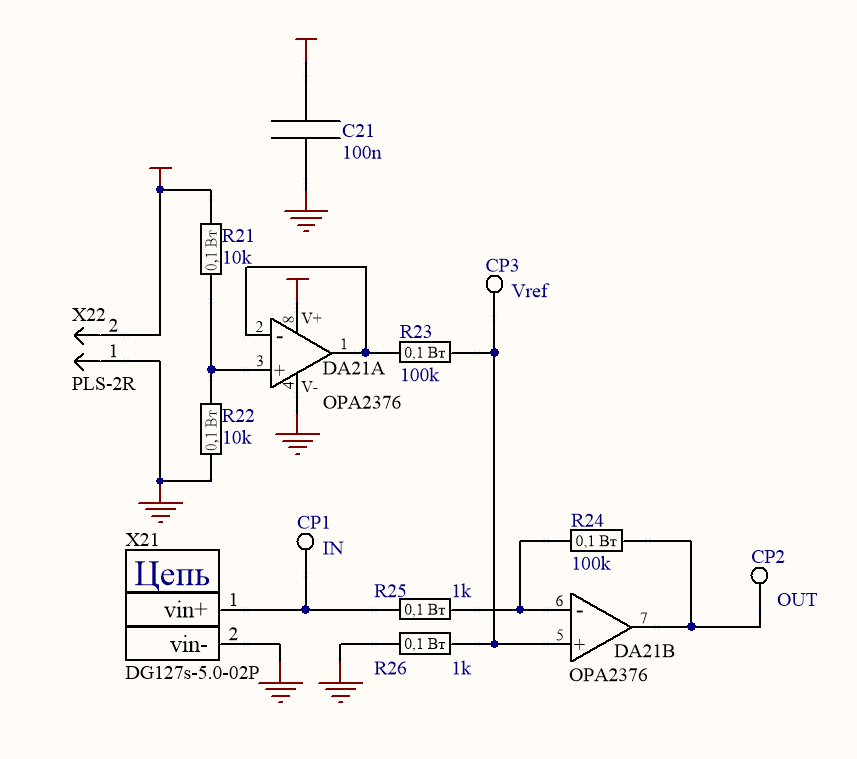
\includegraphics[scale = 0.7]{ris414.png}
\caption{Схема установки для измерения времен восстановления после перегрузки}
\label{ris:414}
\end{figure}

На этой схеме первый ОУ в корпусе DA21A задает стабильные 2,5 В, полученные с делителя R21, R22 с 
коэффициентом деления равным 2, на неинвертирующем входе второго ОУ в корпусе DA21B, включенного по схеме
инвертирующего усилителя с коэффициентом усиления равным -100. В данном эксперименте на вход подается 
сигнал с функционального генератора Tektronix AFG 31000.


Осцилограммы измерения время восстановления после положительной перегрузки (Positive Over-Voltage Recovery) 
и после отрицательной перегрузки (Negative Over-Voltage Recovery) для вышеперечисленных операционных усилителей
представлены на рисунках \ref{ris:415} - \ref{ris:426}. На всех рисунках желтый сигнал - на инвертирующем 
входе ОУ, а розовый - сигнал с выхода ОУ. Развертка по вертикали у входного сигнала -- 50 мВ/деление, 
у выходного 1 В/деление. 

\begin{figure}[H]
\centering
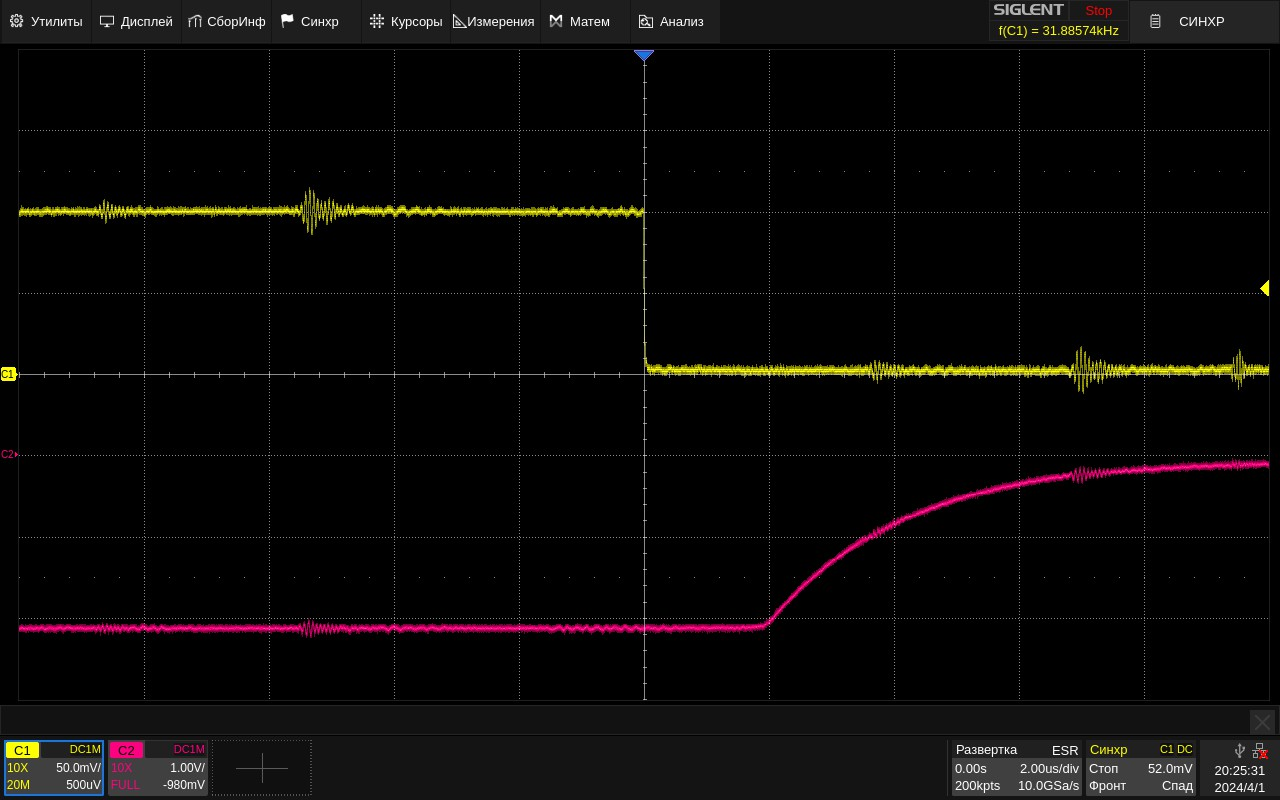
\includegraphics[scale = 0.4]{AD8606_NOR.jpg}
\caption{Negative Over-Voltage Recovery у AD8606, развертка 2 мкс/деление}
\label{ris:415}
\end{figure}

\begin{figure}[H]
\centering
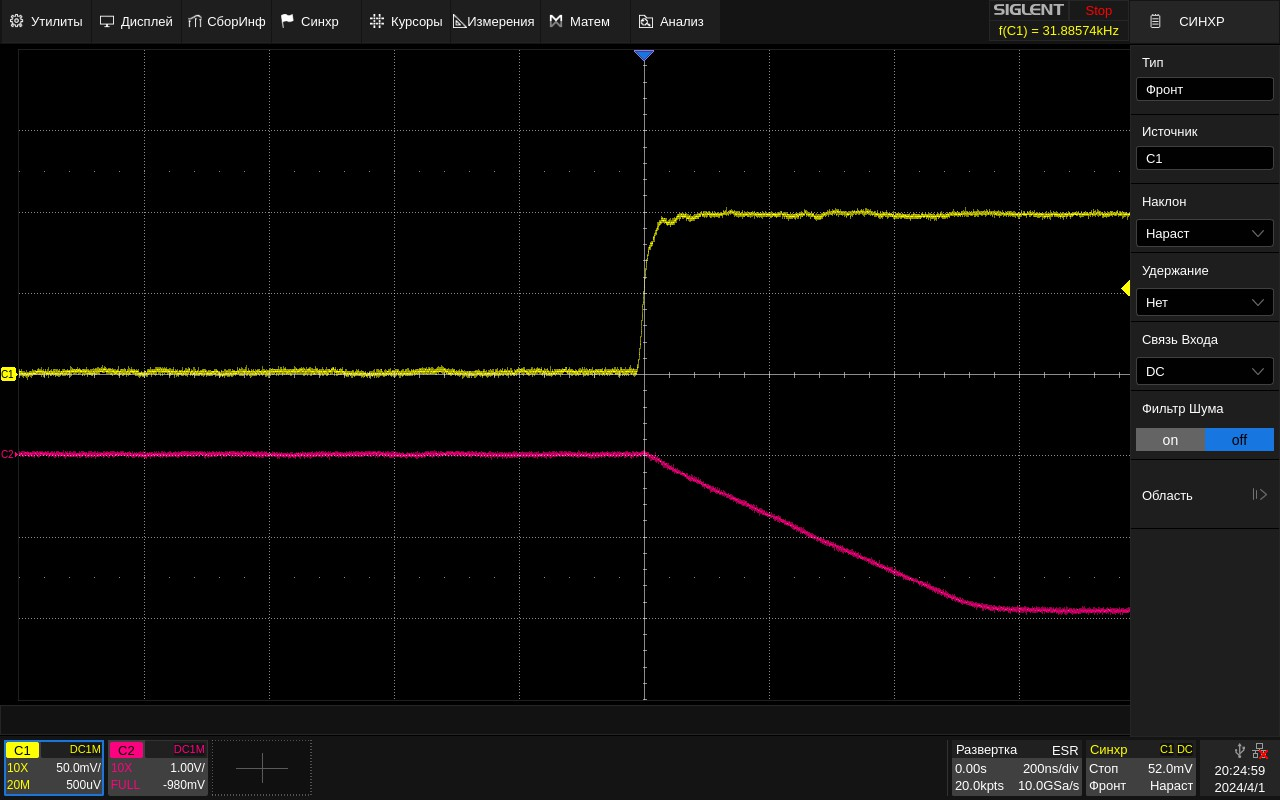
\includegraphics[scale = 0.4]{AD8606_POR.jpg}
\caption{Positive Over-Voltage Recovery у AD8606, развертка 200нс/деление}
\label{ris:416}
\end{figure}

У AD8606 Negative Over-Voltage Recovery (здесь и далее NOR) примерно равно 5 мкс,
 Positive Over-Voltage Recovery (здесь и далее POR) примерно равно 450 нс.

\begin{figure}[H]
\centering
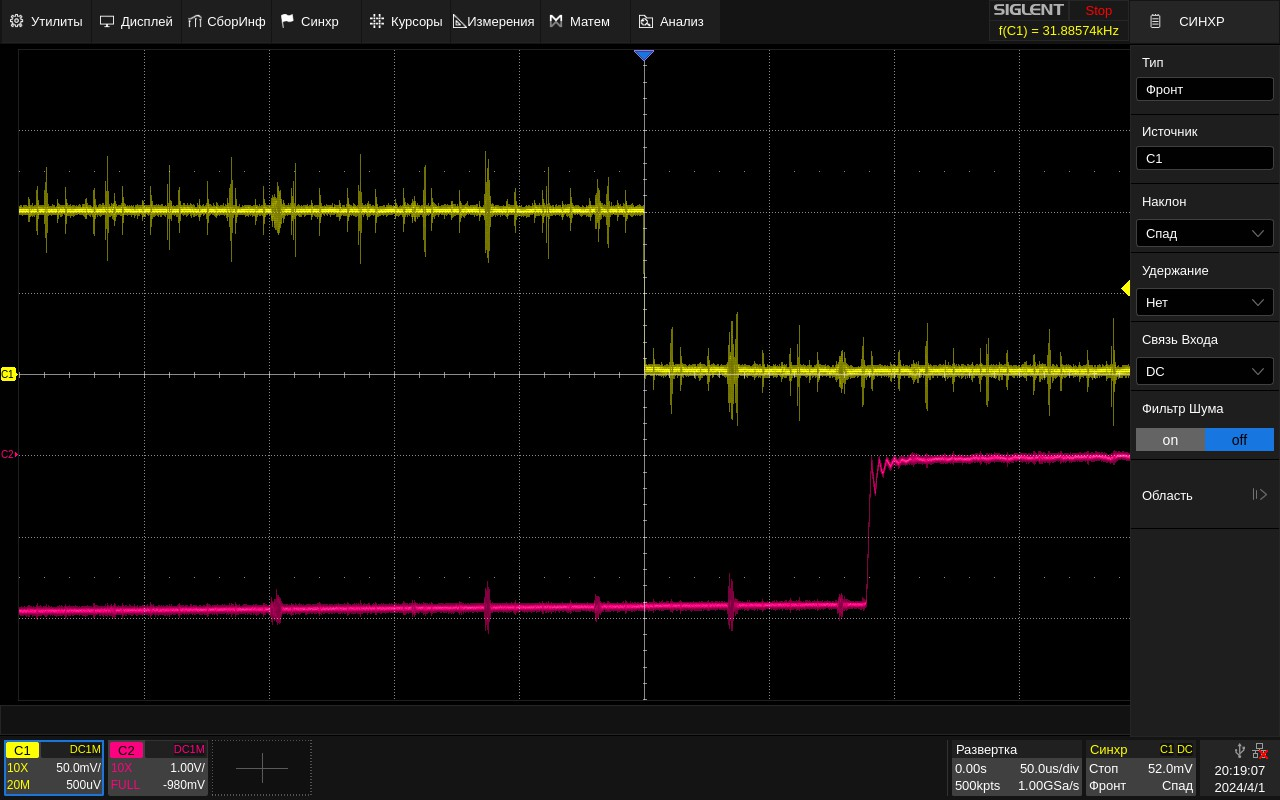
\includegraphics[scale = 0.4]{OPA2376 Fulihao_NOR.jpg}
\caption{Negative Over-Voltage Recovery у OPA2376 Fulihao, развертка 50 мкс/деление}
\label{ris:417}
\end{figure}

\begin{figure}[H]
\centering
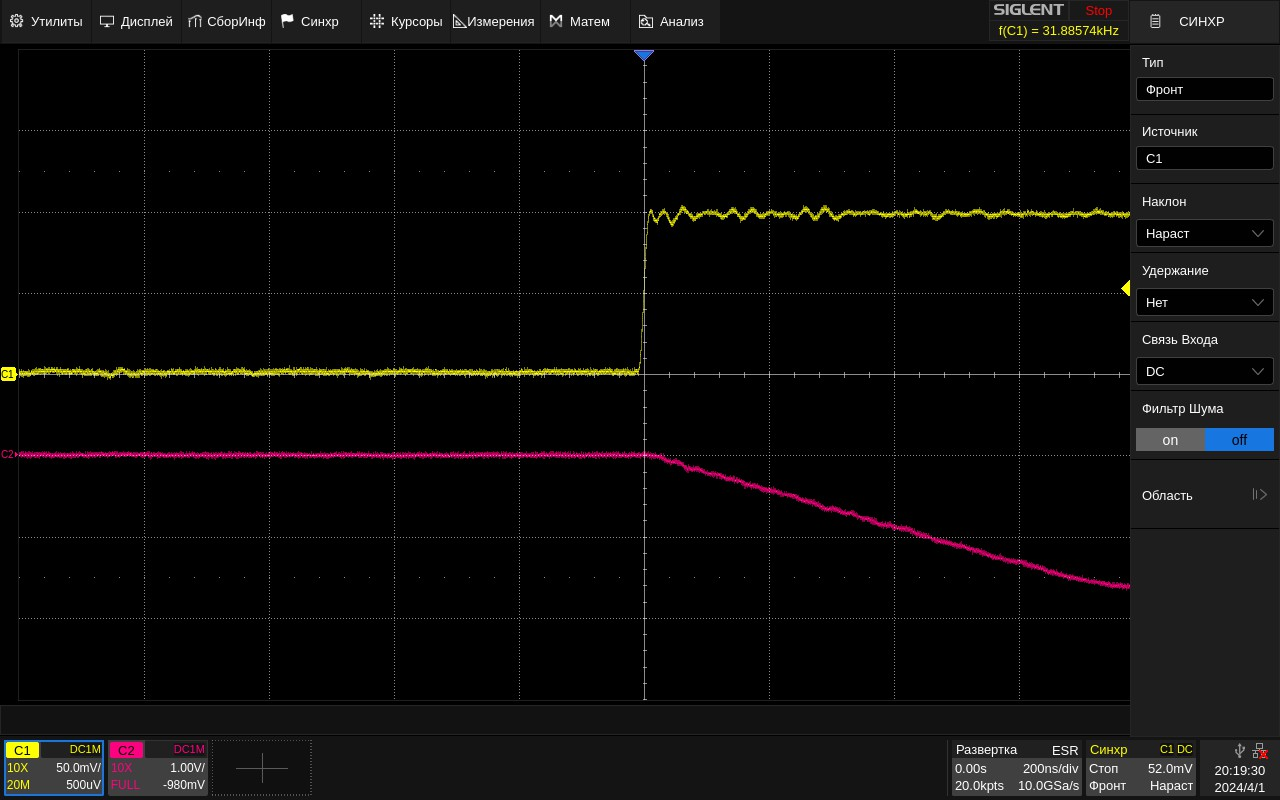
\includegraphics[scale = 0.4]{OPA2376 Fulihao_POR.jpg}
\caption{Positive Over-Voltage Recovery у OPA2376 Fulihao, развертка 200 нс/деление}
\label{ris:418}
\end{figure}

У OPA2376 Fulihao NOR примерно равно 90 мкс,
POR примерно равно 600 нс.

\begin{figure}[H]
\centering
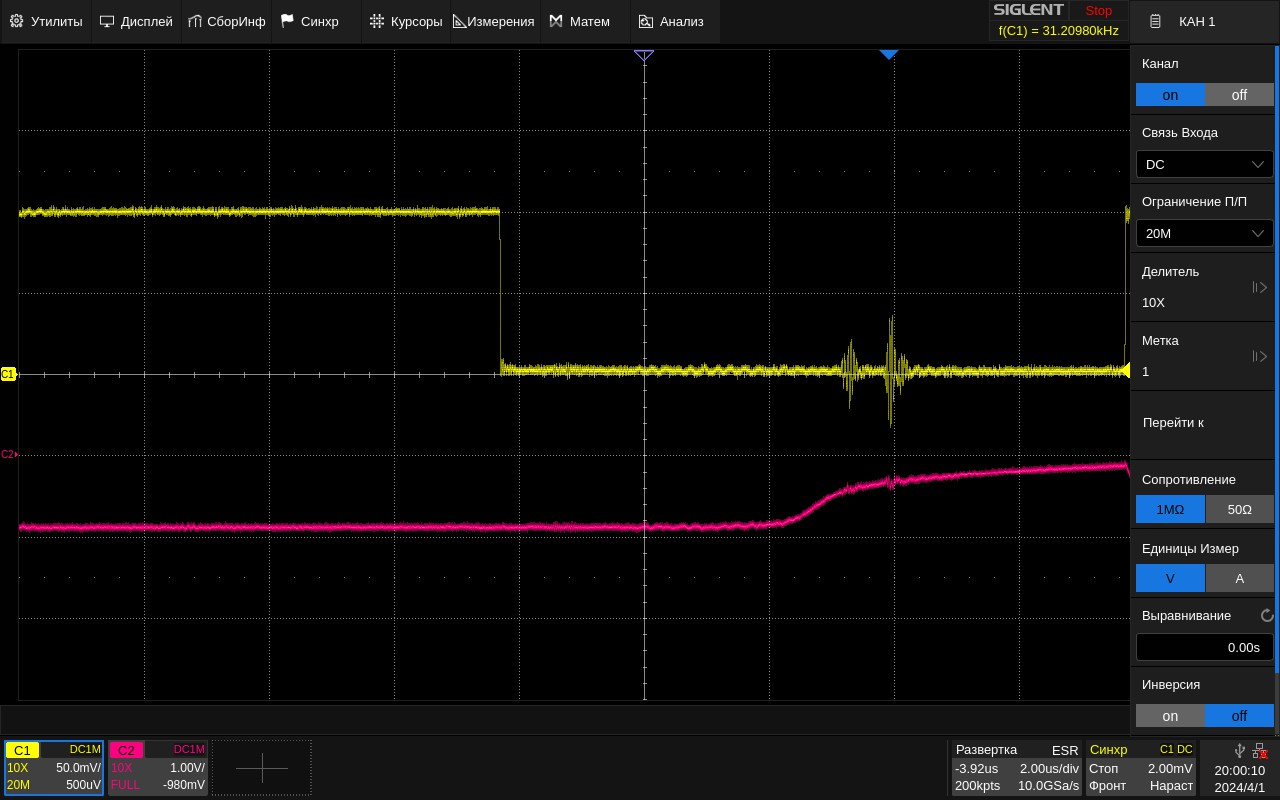
\includegraphics[scale = 0.4]{OPA2376 TI_NOR.jpg}
\caption{Negative Over-Voltage Recovery у OPA2376 TI, развертка 2 мкс/деление}
\label{ris:419}
\end{figure}

\begin{figure}[H]
\centering
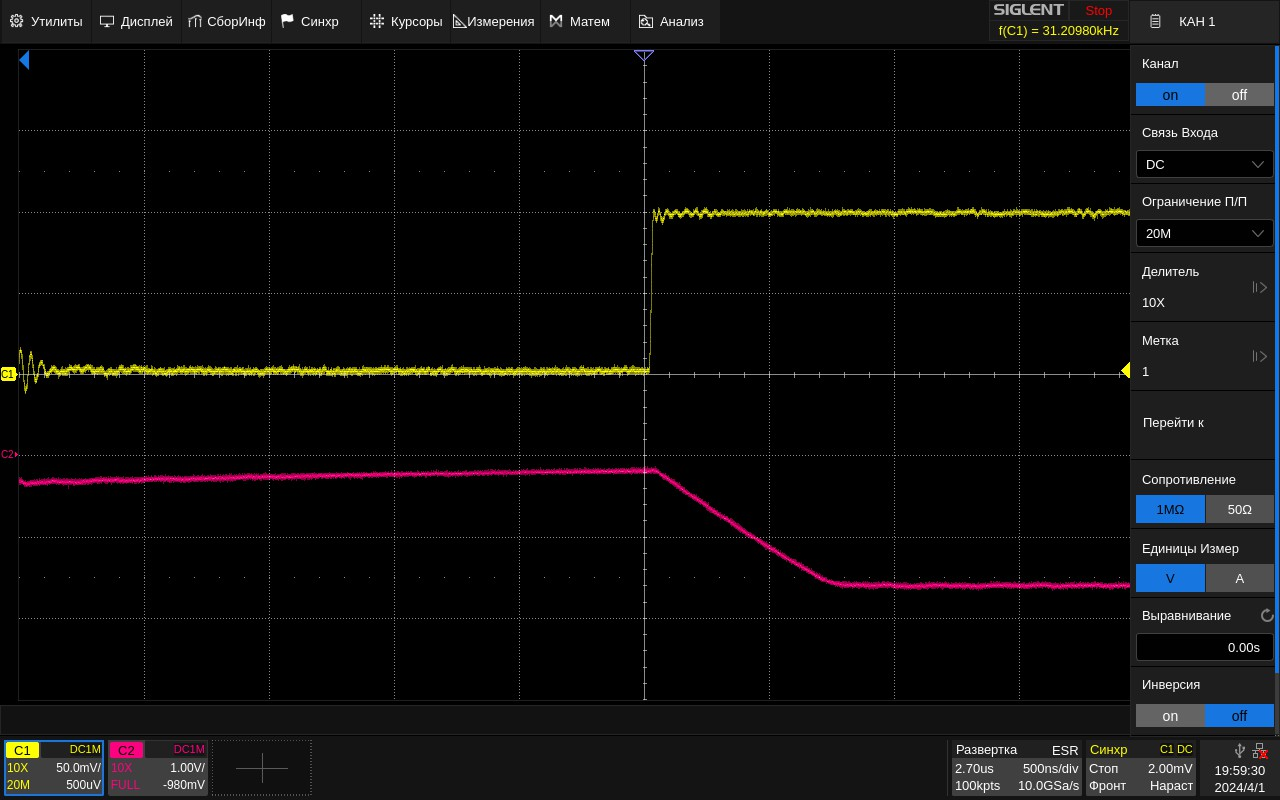
\includegraphics[scale = 0.4]{OPA2376 TI_POR.jpg}
\caption{Positive Over-Voltage Recovery у OPA2376 TI, развертка 500 нс/деление}
\label{ris:420}
\end{figure}

У OPA2376 TI NOR примерно равно 4,25 мкс, 
POR примерно равно 600 нс. 

\begin{figure}[H]
\centering
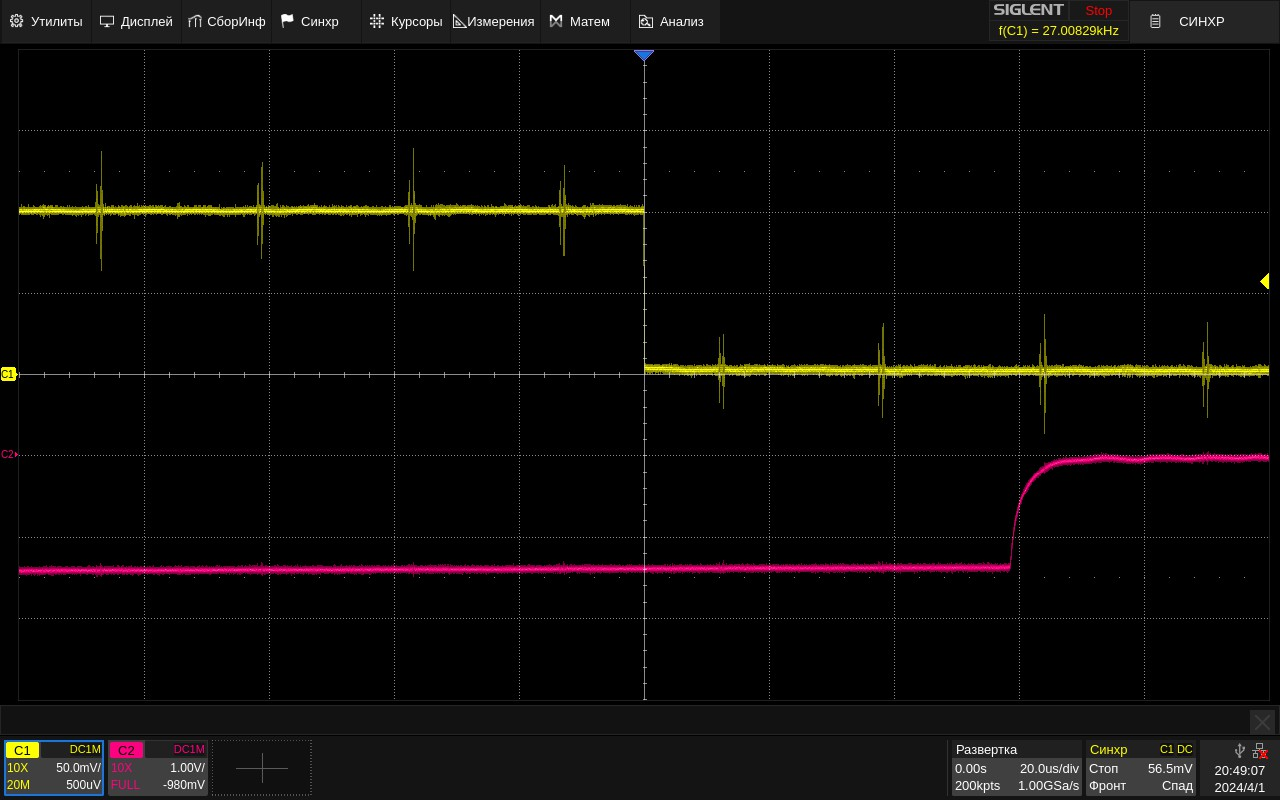
\includegraphics[scale = 0.4]{RS8552_NOR.jpg}
\caption{Negative Over-Voltage Recovery у RS8552, развертка 20 мкс/деление}
\label{ris:421}
\end{figure}

\begin{figure}[H]
\centering
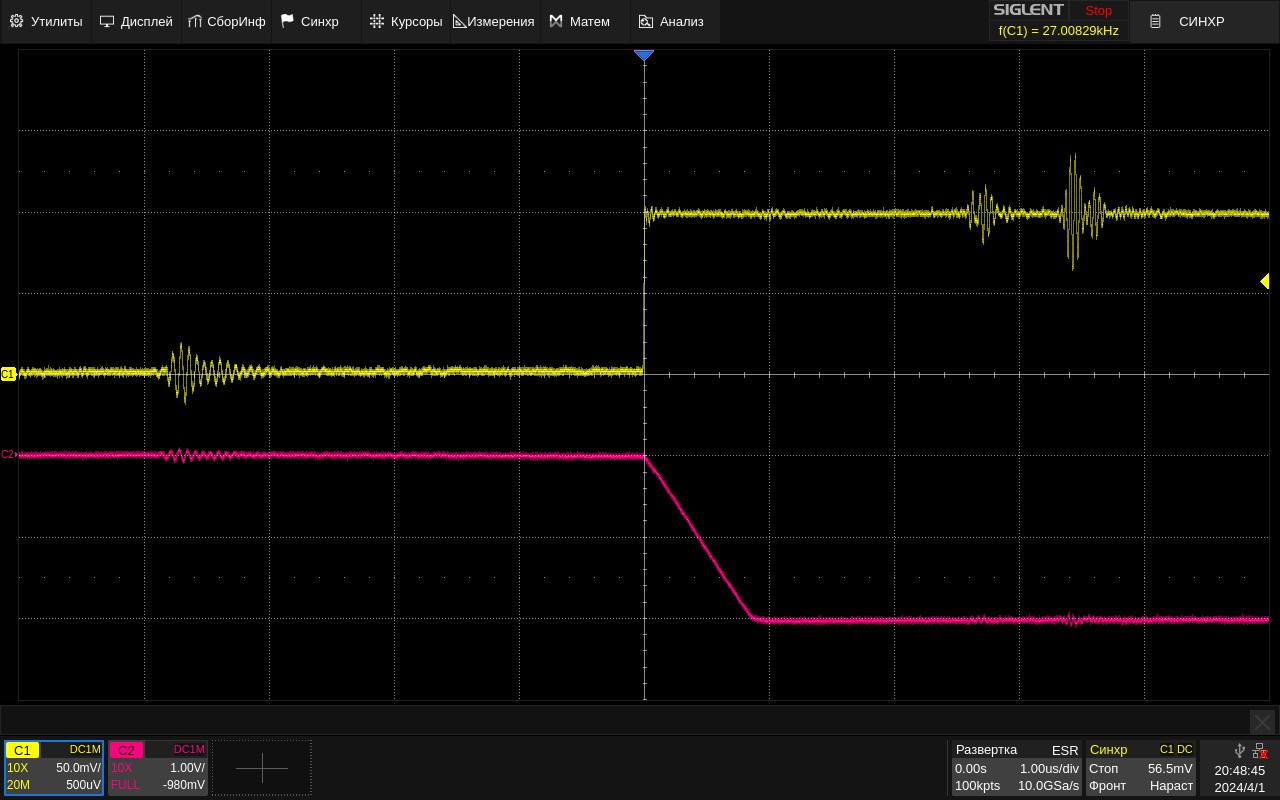
\includegraphics[scale = 0.4]{RS8552_POR_2.jpg}
\caption{Positive Over-Voltage Recovery у RS8552, развертка 1 мкс/деление}
\label{ris:422}
\end{figure}

У RS8552 NOR примерно равно 60 мкс, 
POR примерно равно 750 нс.

\begin{figure}[H]
\centering
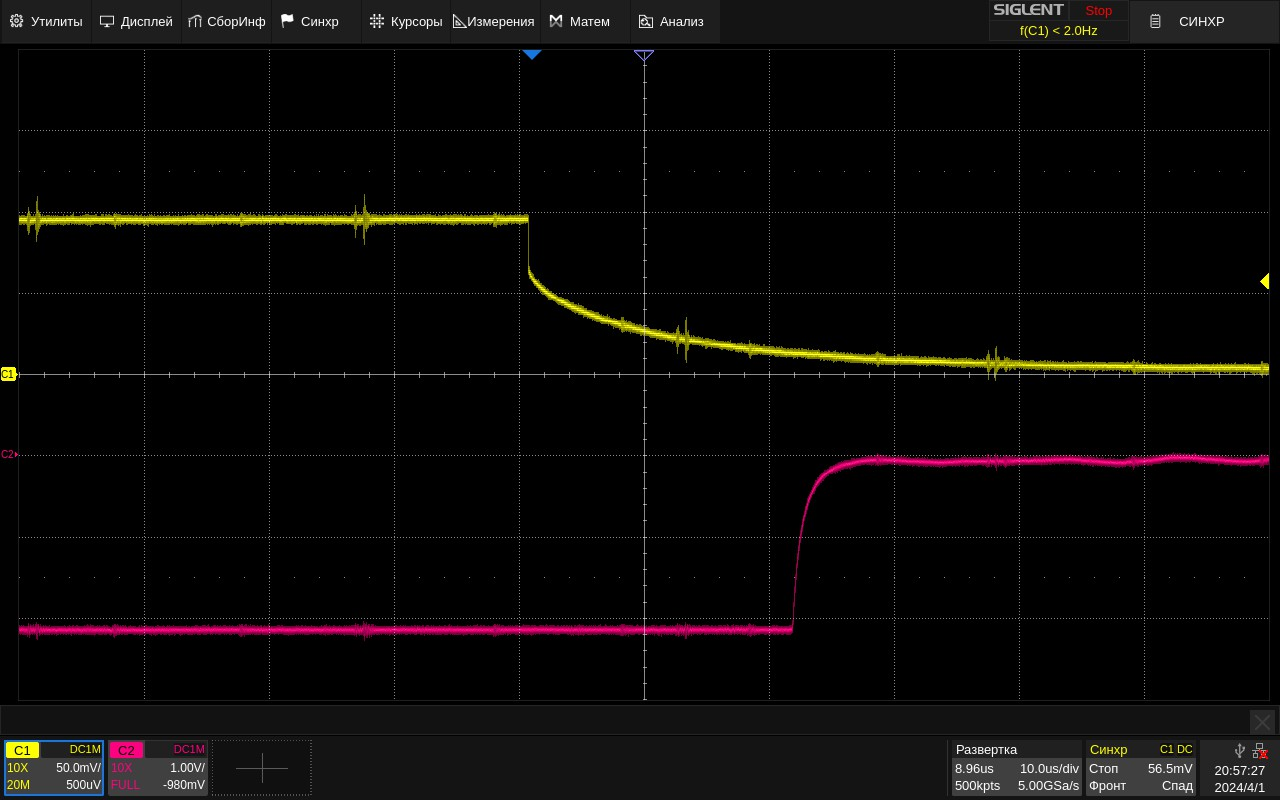
\includegraphics[scale = 0.4]{RS8562_NOR.jpg}
\caption{Negative Over-Voltage Recovery у RS8562, развертка 10 мкс/деление}
\label{ris:423}
\end{figure}

\begin{figure}[H]
\centering
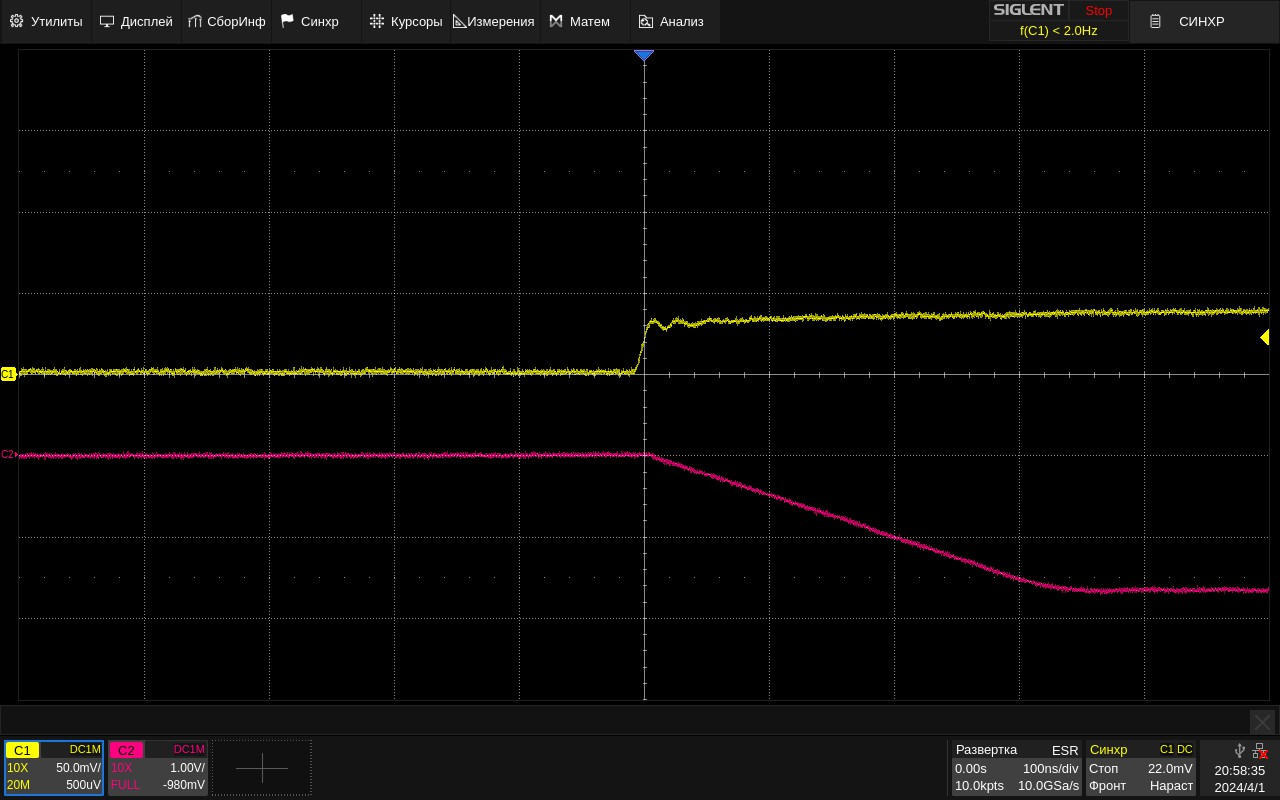
\includegraphics[scale = 0.4]{RS8562_POR_2.jpg}
\caption{Positive Over-Voltage Recovery у RS8562, развертка 100 нс/деление}
\label{ris:424}
\end{figure}

У RS8562 NOR примерно равно 22,5 мкс, 
POR примерно равно 300 нс.

\begin{figure}[H]
\centering
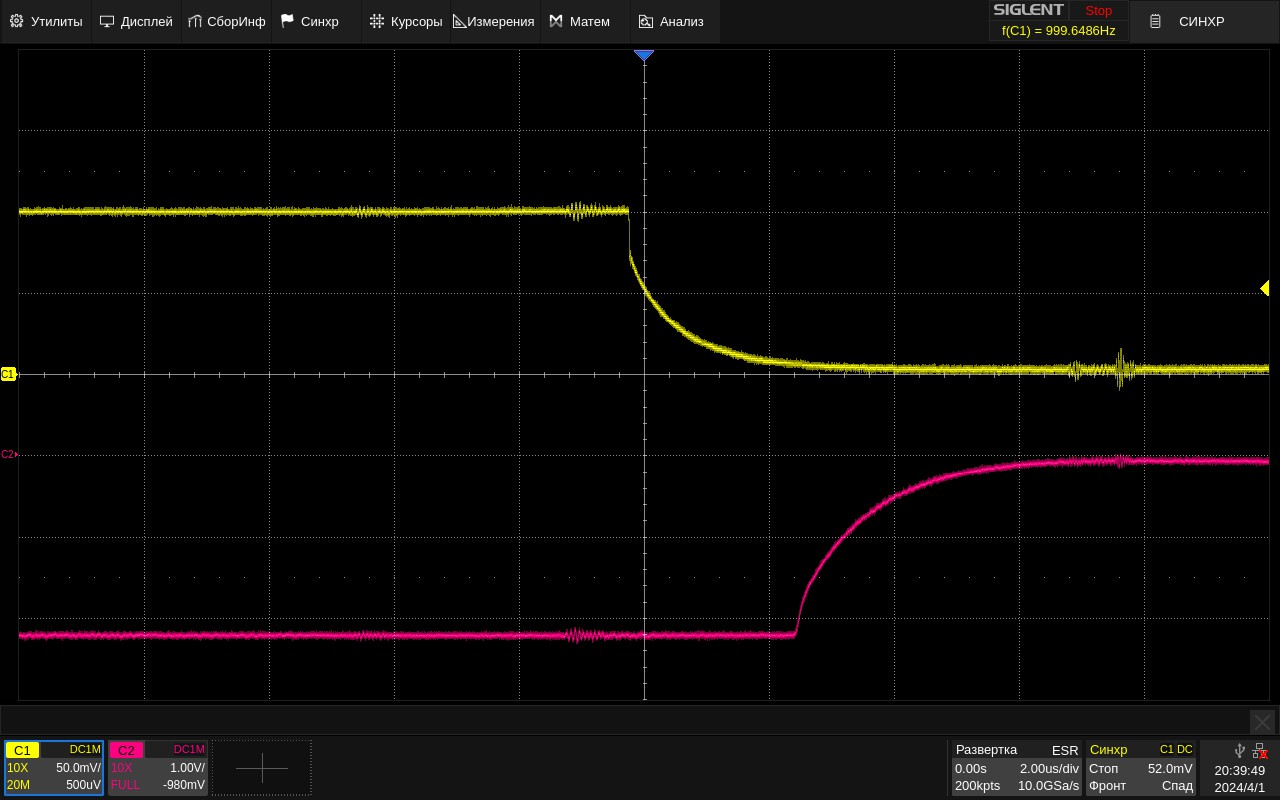
\includegraphics[scale = 0.4]{TP2312_NOR.jpg}
\caption{Negative Over-Voltage Recovery у TP2312, развертка 2 мкс/деление}
\label{ris:425}
\end{figure}

\begin{figure}[H]
\centering
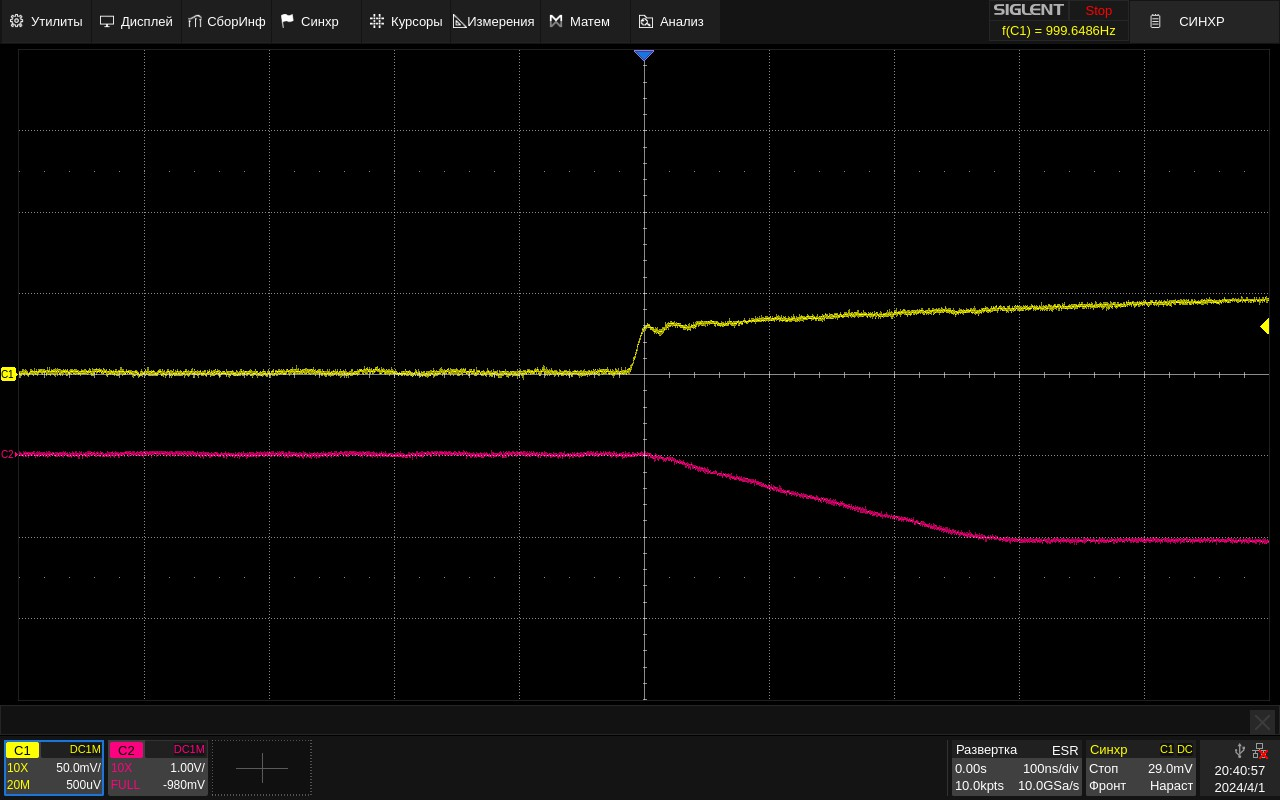
\includegraphics[scale = 0.4]{TP2312_POR_2.jpg}
\caption{Positive Over-Voltage Recovery у TP2312, развертка 100 нс/деление}
\label{ris:426}
\end{figure}

У TP2312 NOR примерно равно 2,25 мкс,
POR примерно равно 200 нс.

Можно заметить разительную разницу во временах восстановления после отрицательной перегрузки у OPA2376 от 
разных производителей. Разница составляет больше, чем в 20 раз. Это свидетельствует о том, что OPA2376 от 
Fulihao на самом деле не etrim, а чоппер-стабилизированный, ведь именно для этого типа ОУ характерны такие 
времена восстановления.
Это не только делает OPA2376 от Fulihao непригодным к использованию для наших целей, но и заставляет 
внимательнее следить в целом за всеми заказанными OPA2376, особенно от китайских производителей.

По результатам всех проведенных измерений выбор основного измерительного операционного усилителя пал на 
TP2312, у него одно из самых малых напряжений смещений, не было замечено нестабильностей в работе, 
а так же у него оказались самые маленькие времена восстановлений после перегрузки. Так же стоит отметить 
его доступность в РФ.

\subsection{Измерительный шунт}
\hspace{1cm} 

Важным элементом в измерительной схеме выступает шунт, — его физические свойства, 
такие как сопротивление, максимальная мощность или температурный коэффициент, 
сильно влияют на точность всего измерения. Поэтому выбор подходящей модели шунтирующего резистора 
важен для корректных измерений. Например, слишком высокое сопротивление шунта может привести к 
значительному падению значения выходного напряжения ниже допустимого уровня, что приведет к снижению 
эффективности устройства. Кроме того, большая мощность, рассеиваемая на шунте, повысит его температуру, 
что дестабилизирует его рабочие параметры и ухудшит точность измерений. Так же высокий температурный 
коэффициент сопротивления (ТКС) сделает всю измерительную часть нетермостабильной, что так же нарушит 
корректность измерений. Этот параметр описывает повышение значений сопротивления элемента в зависимости от
его температуры -- чем больше ТКС, тем ниже точность измерения.

Другой важной характеристикой шунтирующего резистора является тепловой коэффициент ЭДС. На стыке 
соединений двух разных металлов создается электродвижущая сила порядка микровольт. Величина этой 
силы (и создаваемое ею напряжение) изменяется в зависимости от температуры. Эти изменения описываются 
тепловым коэффициентом (чаще всего выражают в мкВ/°С). Шунтирующие резисторы могут работать в широком 
диапазоне измерений -- при измерении очень малых токов дополнительное напряжение, вызванное фактором 
ЭДС, может значительно исказить результаты.

Для того чтобы значение тока измерялось с хорошей точностью следует отказаться от упрощенной модели 
состоящей из одного значения сопротивления, заменив ее более сложной, хотя и более реалистичной моделью, 
состоящей из трех последовательно соединенных сопротивлений. Это номинальное и двухкомпонентное 
сопротивление. В случае обычных резисторов сопротивления выводов имеют пренебрежимо малые значения, 
в случае шунтирующих, характеризующихся очень малыми значениями номинального сопротивления, 
эти дополнительные паразитные параметры вносят существенный вклад в работу, а игнорирование их 
влияния приводит к увеличению погрешности измерения. Схема замещения шунта изображена на рисунке 
\ref{ris:427}.

\begin{figure}[H]
\centering
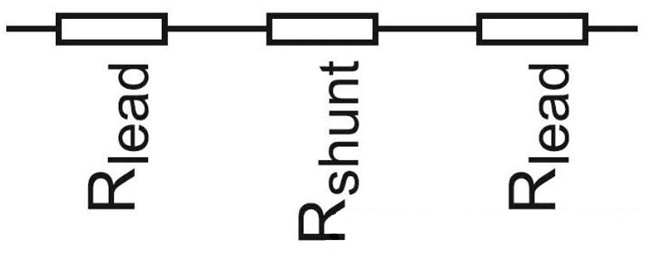
\includegraphics[scale = 1]{ris427.png}
\caption{Схема замещения шунтирующего резистора}
\label{ris:427}
\end{figure}

Для достижения требуемой точности измерения тока в 0,5\% на разных диапазонах измеряемого тока, 
требуется использовать шунты разного номинала. С учетом требований к устройству, сформированных в главе 1,
номиналы шунтов, которых хватит для покрытия всего измеряемого диапазона, были выбраны 
0,01 Ом, 1 Ом, и 100 Ом. С точки зрения подбора ЭКБ самыми проблемными являются шунты на 0,01 Ом. 
В ходе поиска и подбора шунтов выбор пал на серию WSL2512 для шунтов 0,01 Ом, так как шунты данной серии
подходят под все требования \cite{GooglePatent:1}. 

\section{Описание схемотехнического решения}
\hspace{1cm}

Даже в рамках измерения по схеме нижнего плеча существуют разные решения. Расмотрим рисунки \ref{ris:428} --
\ref{ris:429}.

\begin{figure}[H]
\centering
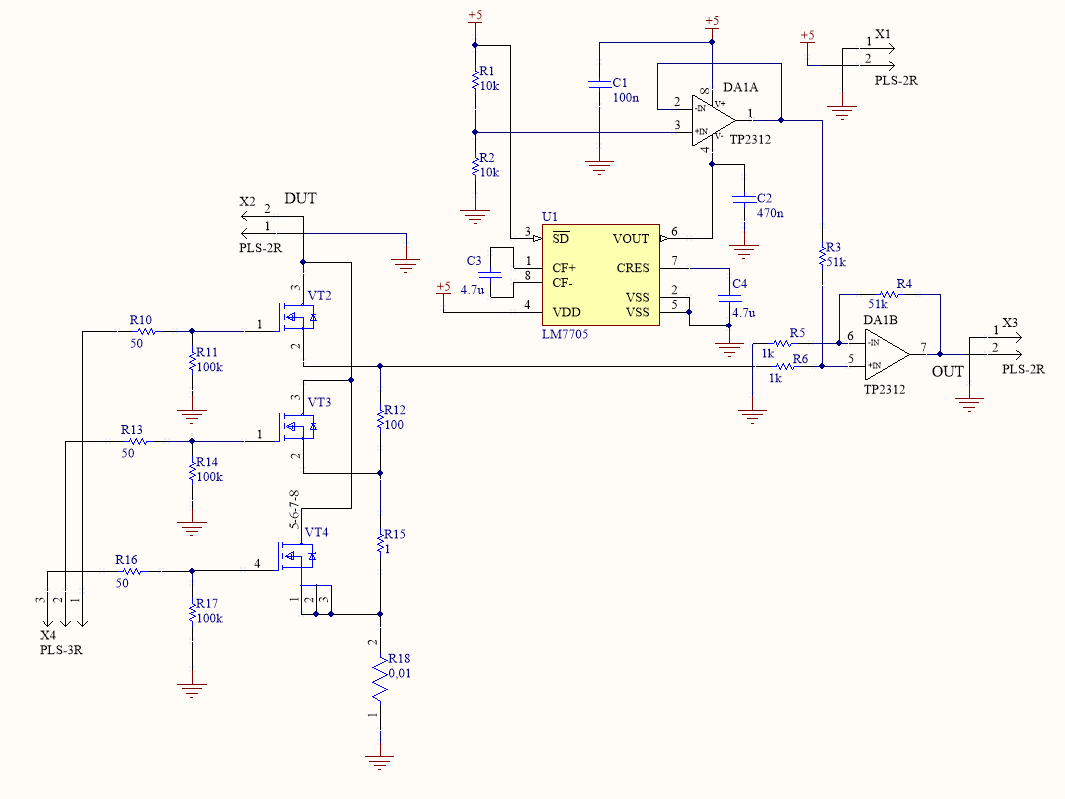
\includegraphics[scale = 0.58]{Meas_LM7705.png}
\caption{Схема измерения с LM7705}
\label{ris:428}
\end{figure}


\begin{figure}[H]
\centering
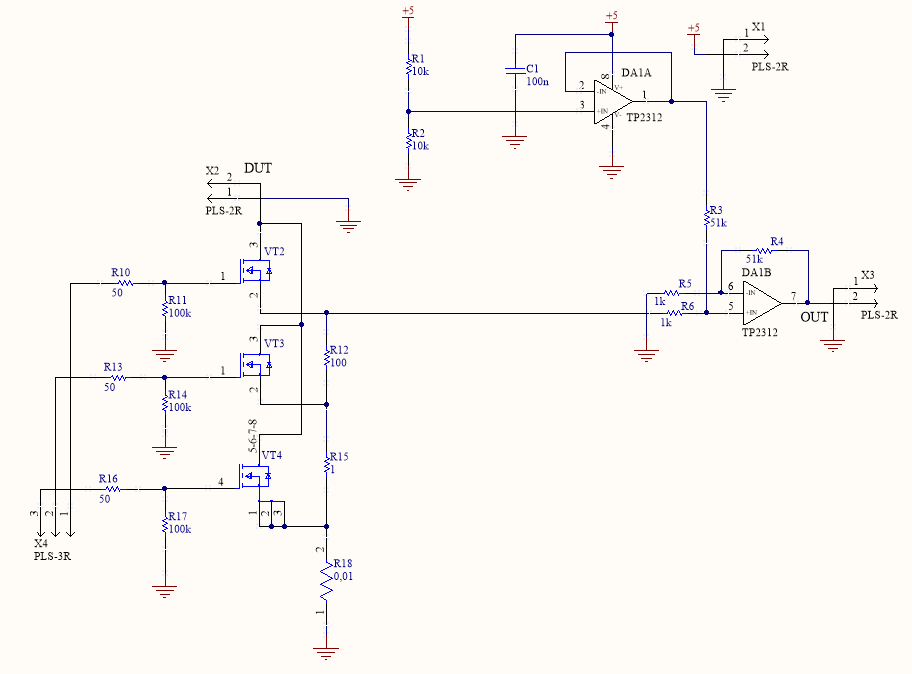
\includegraphics[scale = 0.63]{Meas_whithout_LM7705.png}
\caption{Схема измерения без LM7705}
\label{ris:429}
\end{figure}

В основе данных схем лежит операционный усилитель DA1B, включенный по схеме дифференциального усилителя с 
коэффициентом усиления 51, который задан резисторами R3-R6. Суть его работы заключается в усилении разницы 
напряжений между входами. На неинвертирующий вход подано смещение 2,5 В, которое задается делителем R1, R2 и 
стабилизируется ОУ DA1A, включенным по схеме повторителя. С разъема Х3 снимается выходное усиленное напряжение. 

Разъем X2 предназначен для подключения источника постоянного тока, имитирующего ток потребления отлаживаемых устройств. 
Транзисторы VT2 -- VT4, включенные по ключевой схеме задают, при подаче на их затвор высокого уровня напряжения,
через какие шунты R12, R15, R18 протечет ток с разъема Х2, создавая определенное падение напряжения. 
Очевидно, что при включении транзистора VT2 ток будет протекать через
все шунты, общим сопротивлением 101,01 Ом, создавая падение напряжения, согласно закону Ома, равное 
$U_{drop} = I_{source} \cdot R_{shunt} = 101,01 \cdot I_{source}$. При включении транзистора VT3 падение напряжения
на шунтах будет составлять $1,01 \cdot I_{source}$, и $0,01 \cdot I_{source}$ при включении транзистора VT4.

Так же стоит отметить, что неиспользуемые резисторы шунта всегда подключены к R6 и вносят некоторую погрешность в 
передаточную функцию. 
% Если успею, то расчитать вносимую погрешность

Резисторы R10, R11, R13, R14, R16, R17 предназначены для защиты управляющего транзисторами элемента от короткого
замыкания, путем ограничения протекающего тока. Это работает следующим образом: у каждого МОП-транзистора, 
из-за наличия у него pn-перехода, имеются
паразитные емкости $C_{gate-source}$, $C_{gate-drain}$, $C_{drain-source}$. Не так важно их значение, как то, что
переходная характеристика любой емкости в начальный момент зарядки имеет импеданс близкий к нулю, что 
показано на рисунке \ref{ris:430}

\begin{figure}[H]
\centering
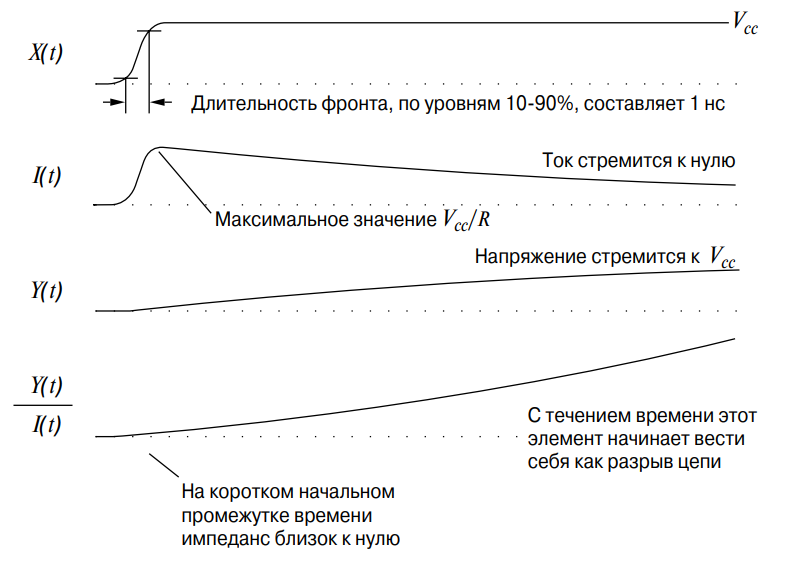
\includegraphics[scale = 0.55]{C_transtion.png}
\caption{Переходная характеристика идеального конденсатора}
\label{ris:430}
\end{figure}

, где из-за очень маленького начального соотношения $\frac{Y_{(t)}}{I_{(t)}}$, в момент возникновения ступенчатого
скачка напряжения, через емкость протекает очень большой ток, ограниченный только сопротивлением
дорожек на печатной плате и сопротивлением выводов конденсаторов, которые из-за конструктивных особенностей очень
малы. А большой ток, как известно, вызывает короткое замыкание \cite{Howard J: Start Black Magic}.

Единственное отличие между схемами в наличии или отсутствии на них микросхемы LM7705 с обвязкой. Эта микросхема
предназначена для обеспечения смещения в -0,23 В на минусе питания ОУ, что необходимо для ухода из зоны с плохим 
напряжением смещения, см. рисунок \ref{ris:411}, а так же для ОУ, которые не являются 
rail-to-rail (или почти являются), позволяет получить на выходе ровно 0 В, не напряжение смещения. 
Так как обе рассматриваемых схемы являются двунаправленными, а для них оба преимущества, которые дает LM7705 не так 
важны, то в итоге за основу подсистемы измерения энергопотребления была выбрана схема, изображенная на рисунке 
\ref{ris:429}.

После подбора основных компонентов подсистемы измерения энергопотребления и анализа деталей схемотехнического
исполнения, можно составить схему электрическую принципиальную измерительной части отладчика, 
которая изображена на рисунке \ref{ris:431}.

\begin{figure}[H]
\centering
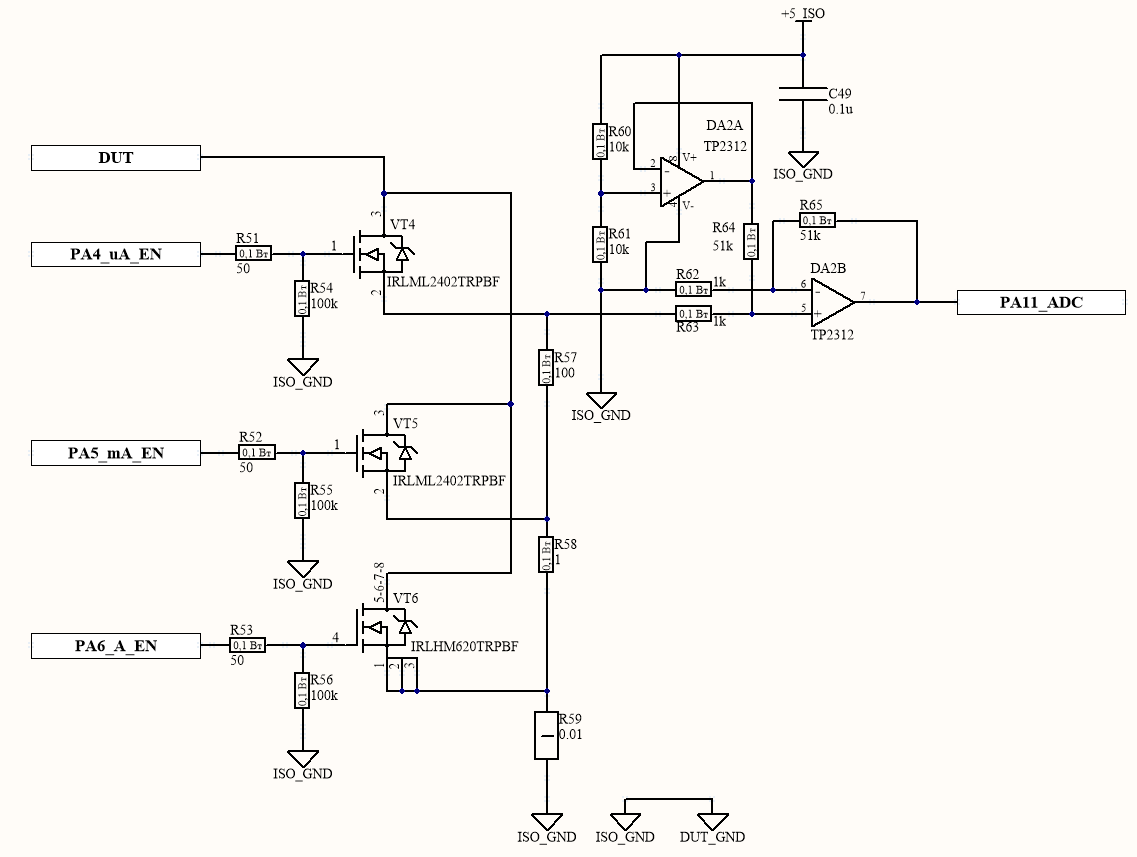
\includegraphics[scale = 0.6]{ris431.png}
\caption{Итоговая схема подсистемы измерения энергопотребления}
\label{ris:431}
\end{figure}

Стоит обговорить еще раз принцип ее работы, учитывая специфику общей схемы. 
С порта DUT подается потребляемый отлаживаемым устройством ток, который дальше в зависимости 
от того, какой транзистор открыт, протекает через шунты R57, R58, R59, создавая тем самым падение напряжения, 
которое попадает на неинверсный вход операционного усилителя DA2B и разница между входами ОУ усиливается в 51 
раз и подается на внутренний 12-битный АЦП микроконтроллера STM32F107, который оцифровывает значение  напряжения.

Сигнал на порты PA4\_uA\_EN, PA5\_mA\_EN, PA6\_A\_EN приходит с микроконтроллера и открывает соответствующий 
транзистор, тем самым реализуя переключение диапазонов измеряемого тока.

Конденсатор C49 является фильтрующим по питанию. 

Повторитель, реализованный на DA2A, задает смещение в 2,5 В на неинверсном входе ОУ DA2B, тем самым позволяя нам 
измерять как положительные, так и отрицательные значения токов. Так реализуется двунаправленный измеритель тока. 